\section{Asymptotic Order of Growth}

\subsection{Brute Force}
For many non-trivial problems, there is a natural brute force search algorithm that checks every possible solution, usually taking $2^{n}$.
\subsection{Polynomial Running Time}
This is the most desirable running time of any algorithm because it scales with ease at the increment of the input size.\\An algorithm can be defined as poly-time if the following property holds:

\[ \exists c > 0, \exists d >0, \; such \; that \; \forall n \in INPUT \; the \; running \; time \; is \; bounded \; by\; cn^{d} \]

We can now give the following definition of efficiency:

\[ An \; algorithm \; is \; efficient \; if \; it \; is \; poly-time.\]

When discussing the running time of a deterministic algorithm is important to take into account the worst-case scenario because, in doing that, the running time is guaranteed $\forall n \in INPUT.$ There are some exception to this rule, when the worst-case scenario is very rare.\\\\
When discussing of probabilistic algorithm we need, instead, to reason upon the expected running time.

\subsection{Big-O Notation}

Assuming we have an algorithm rappresented by the function:
\[ T(n) = 1.6n^{2} + 3.5n+8\]
We want a way to express the growing rate in a way that is insensitive to constant factors and low-ordered terms, in fact It can be said that T(n) grows like $\mathcal{O}(n^{2})$.\\

\begin{itemize}
    \item The lower bound $\mathcal{O}$\\
          We can say that T(n) is $\mathcal{O}{(f(n))}$ if $\exists c > 0, \exists n_{0} \geq 0 / \; T(n) \leq cf(n), \; \forall n \geq n_{0}$

          We can give an alternative definition as follow:
          \[ \mathcal{O}{(f(n))} = \lim_{n\to\infty} \frac{T(n)}{F(n)} < \infty\]

          Graphically:

          \begin{figure}[H]
              \centering
              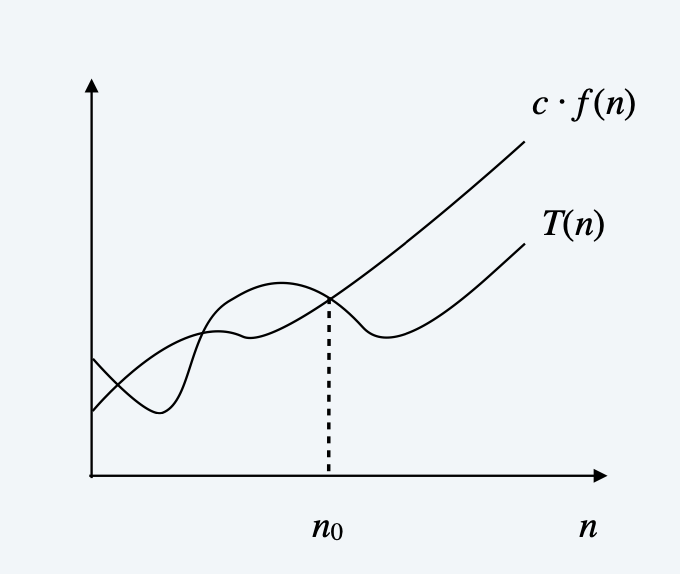
\includegraphics[width=0.4\textwidth ]{on}
          \end{figure}

          Again, going back to our function: $T(n) = 1.6n^{2} + 3.5n+8$,
          \[ T(n) = n^{3}\]
          \[ T(n) = n^{2}\]
          \[ T(n) \neq n\]


    \item The upper bound $\Omega$ \\
          We can say that T(n) is $ \Omega(f(n)) \;if \exists c > 0, \exists n_{0} \geq 0 / \; T(n) \geq cf(n), \; \forall n \geq n_{0}$

          Again, going back to our function: $T(n) = 1.6n^{2} + 3.5n+8$,
          \[ T(n) = \Omega(n)\]
          since $T(n) \leq pn^{2} \leq pn$.\\


          Graphically:

          \begin{figure}[H]
              \centering
              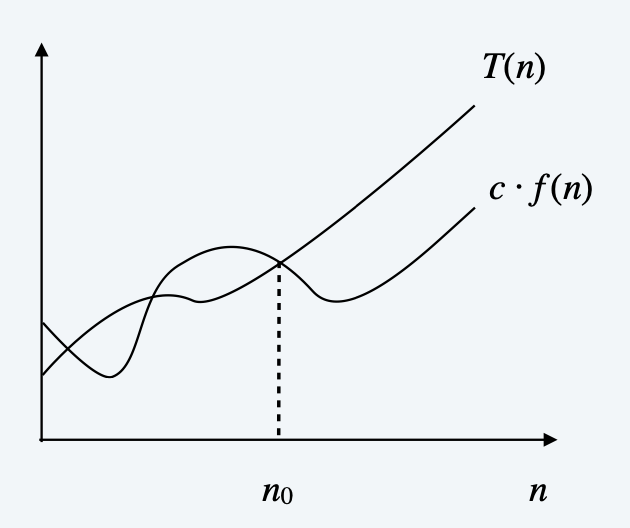
\includegraphics[width=0.4\textwidth ]{omega}
          \end{figure}

    \item The tight bound $\Theta$ \\
          T(n) is $ \Theta(f(n)) \; if \; \exists c_{1} > 0, c_{2}>0 \; and \; \nexists \;n_{0} \; such \; that \; c_{1}f(n) \leq T(n) \leq c_{2} f(n) \; \forall n \geq n_{0}$

          Graphically:

          \begin{figure}[H]
              \centering
              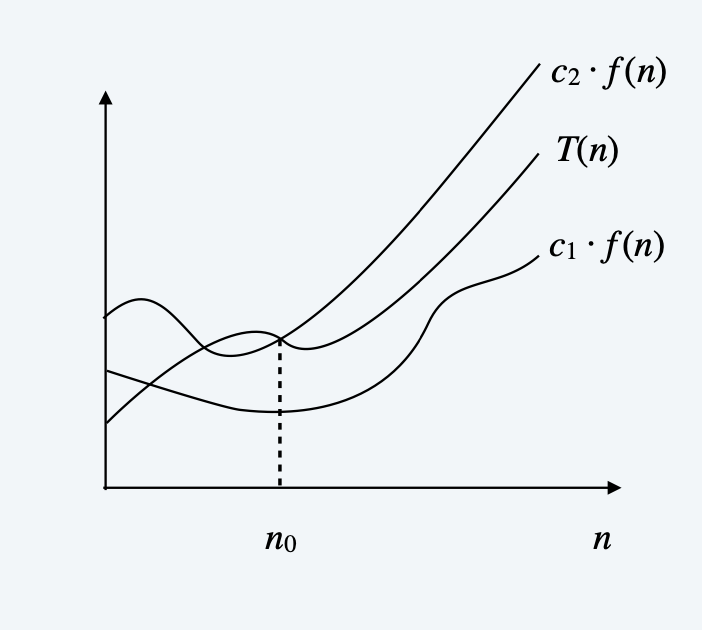
\includegraphics[width=0.4\textwidth ]{tight}
          \end{figure}

    \item {Usefull Properties}\\\\
          Transitivity:
          \[ if \; f = \mathcal{O}{(g)} \; and \; g =\mathcal{O}{(h)}, \; then \;f = \mathcal{O}{(h)}\]
          \[ if \; f = \Omega{(g)} \; and \; g =\Omega{(h)}, \; then \;f = \Omega{(h)}\]\\\\
          Sum of functions:
          Supposing that f and g are two functions such that, for some other function h, we have $f = \mathcal{O}{(h)} \; and \;g = \mathcal{O}{(h)}, \; then \; f + g = \mathcal{O}{(h)}.$

\end{itemize}

\subsection{Common Running Times}

\begin{itemize}

    \item {Linear $\mathcal{O}{(n)}$}\\\\
          The running time is proportional to the input size.\\\\
          Example: finding the maximum into an array.

    \item {Linearithmic time $\mathcal{O}{(nlogn)}$}\\\\
          Very common in divide-and-conquer algorithms, is also the running time of most of the sorting algorithms (ex: MergeSort or HeapSort).\\\\
          Note: if an algorithm A execute n times a sorting operation, let's say n=3, and the sorting operation is still the most computational costly operation in the whole algorithm: then A is still $\mathcal{O}{(nlogn)}$ because $3\mathcal{O}{(nlogn)} \simeq \mathcal {O}{(nlogn)}$.

    \item {Quadratic time $\mathcal{O}{(n^{2})}$}\\\\
          Common when enumerating all pairs of elements, ex: given a list of n points in the plane $(x_{1}, y_{1})$, ..., $(x_{n}, y_{n})$, find the pair that is closest to each other.

    \item {Cubic time $\mathcal{O}{(n^{3})}$}\\\\
          Example:Set disjointness. Given n sets: $S_{1}, ..., S_{n}$ each of which is a subset of 1, 2, ..., n, is there some pair of these which are disjoint?

    \item {Ploynomial time $\mathcal{O}{(n^{k})}$}\\\\
          Example:Independent set of size k: Given a graph, are there k nodes such that no two are joined by an edge? The solution is to enumerate all subsets of k nodes.

    \item {Exponential time}\\\\
          Given a graph, what is maximum cardinality of an independent set? Enumerate all the possible subsets $\Rightarrow \mathcal{O}{(n^{2} 2n)}$

    \item {Sublinear time}\\\\
          Search in a sorted array. Given a sorted array A of n numbers, is a given number x in the array? $ \Rightarrow \mathcal{O}{(logn)}$ Binary search.

          \subsection{Why it Matters}

          \begin{figure}[H]
              \centering
              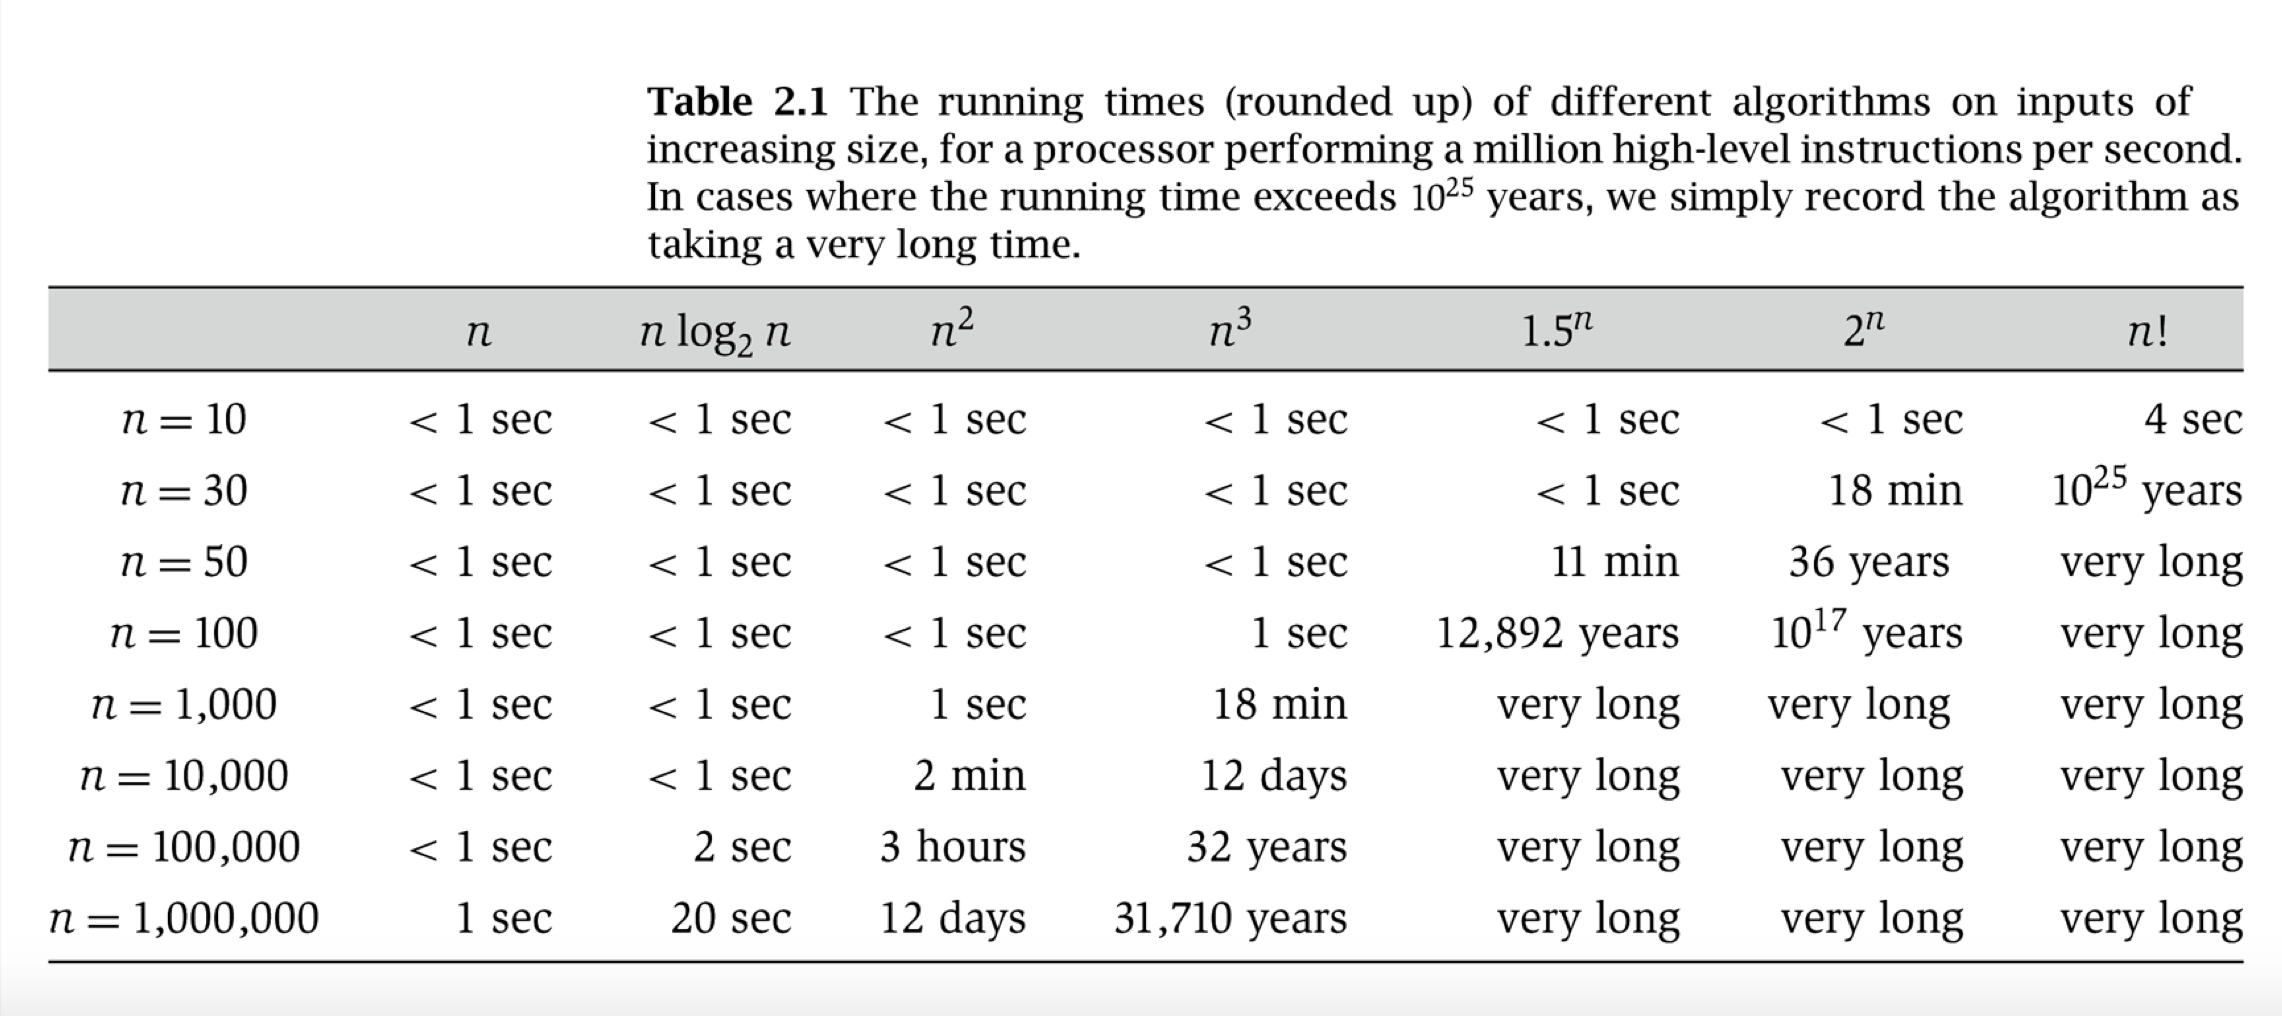
\includegraphics[width=0.7\textwidth ]{running}
              \caption{Comparison of the running times of different complexity algorithms.}
          \end{figure}

          Notice that, as we distance from the linear complexity, for bigger value of $n \in INPUT$, the execution time goes very high, this is bad: let's just say we want to deploy our non-linear algorithm on a distributed system dealing with a lots of records, as they grows, the system could become unable to process them in a feasible time.

          \subsection{The Heap Data Structure}

          Is a balanced binary tree  T(V,E) that satisfy the following property, defining with C the set containing all the children of a node $w_{i}$

          \[ \forall w_{i} \in V, \forall v_{i} \in C, \; key(w_{i}) \leq key(v_{i})\]

          \begin{figure}[H]
              \centering
              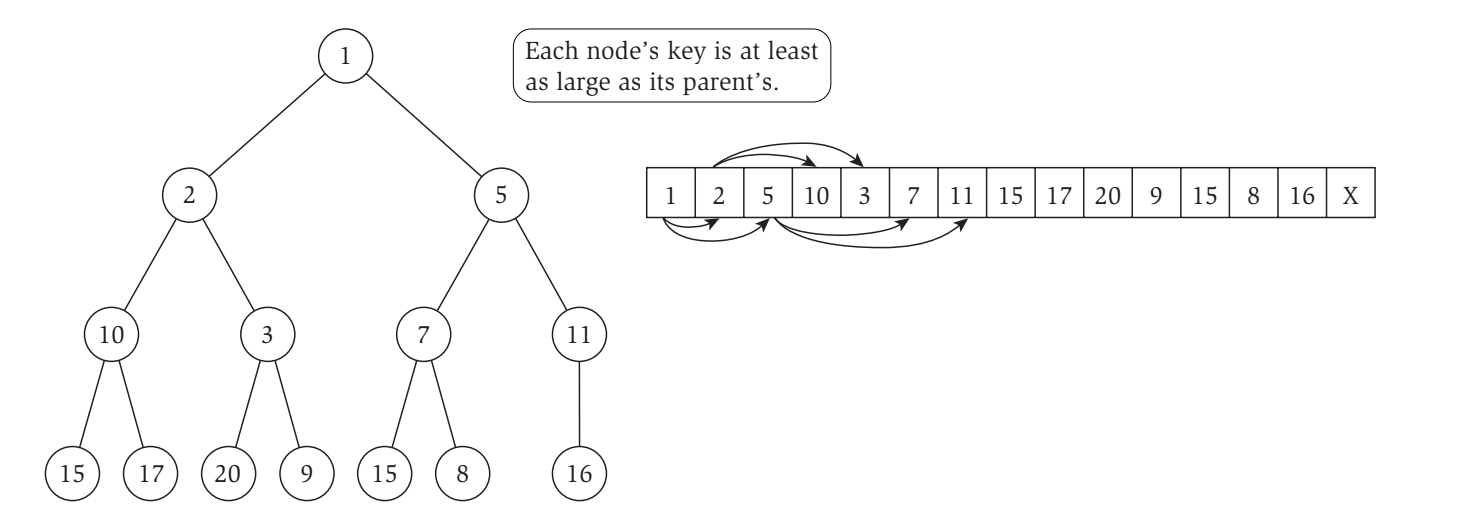
\includegraphics[width=0.7\textwidth ]{heap}
              \caption{An example of heap.}
          \end{figure}

          This data structure is very helpfull, instead of using an array or a list, here are the complexity of some operations involving the heap structure:

          \[ create \; heap =  \mathcal{O}{(n)}\]
          \[ insert \; heap =  \mathcal{O}{(logn)}\]
          \[find \; min =  \mathcal{O}{(1)}\]
          \[delete  =  \mathcal{O}{(logn)}\]

\end{itemize}

\clearpage

